\chapter{Testing and Experimental Results}
\justify

Product development has been completed for the project, and as a result, all functionalities have been thoroughly tested. This chapter presents a comprehensive overview of the features tested, providing screenshots and photographs of hardware to illustrate the outcome of the built systems.

\section{Testing Methodology}
\begin{figure}
    \centering
    \includegraphics[width=0.80\linewidth]{Media/Chapter 6/diagram_testing.png}
    \caption{Testing}
    \label{fig:Testing}
\end{figure}

The testing phase involved various methodologies to ensure the functionality, performance, and reliability of the "Call One" caller ID app. The following testing methods were employed:

\begin{enumerate}
    \item \textbf{Unit Testing:} Testing individual modules and components to verify their correctness and functionality.
    Unit tests cover the smallest parts of code, like individual functions or classes.When the object being tested has any dependencies, you’ll often need to mock them out, as described in the next paragraph.
    
    The great thing about unit tests is that they are quick to write and run. Therefore, as you work, you get fast feedback about whether your tests are passing. Jest even has an option to continuously run tests that are related to code you’re editing: Watch mode.
    
    \item \textbf{Integration Testing:} Testing the integration of different modules and components to ensure they work together seamlessly.
    
    \item \textbf{System Testing:} Testing the entire system as a whole to validate its functionality, performance, and compliance with requirements.

    \item \textbf{Testing and Debugging}: React Native supports various testing and debugging tools, including Jest for unit testing, React Native Debugger for debugging, and tools like Flipper for inspecting app performance and behavior.
    
    
    \item \textbf{User Acceptance Testing (UAT):} Involving users to test the app's usability, user interface, and overall satisfaction.
    
    \item \textbf{Performance Testing:} Assessing the app's performance under various load conditions to ensure optimal performance.
    
    \item \textbf{Security Testing:} Testing the app's security measures, including data encryption, access controls, and authentication protocols.
    
    \item \textbf{Compatibility Testing:} Testing the app's compatibility with different devices, operating systems, and browsers.
    
    \item \textbf{Jest Testing:} Using Jest, a popular JavaScript testing framework, for unit testing JavaScript components and functionalities within the "Call One" app.
    
    \begin{figure}
        \centering
        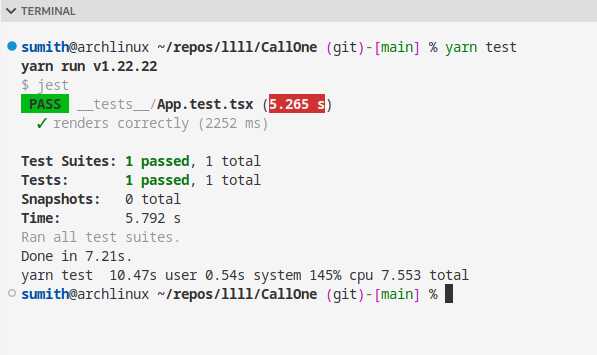
\includegraphics[width=0.90\linewidth]{Media//Chapter 6/jest.png}
        \caption{Jest Testing}
        \label{fig:JestTesting}
    \end{figure}

\end{enumerate}


\section{Experimental Results}

The experimental results of the testing phase demonstrated the following outcomes:

\begin{enumerate}
    \item \textbf{Functionalities Verified:} All functionalities of the "Call One" app were verified and found to be working as expected.
    
    \item \textbf{Performance Optimization:} Performance testing revealed that the app performs optimally under various load conditions, ensuring smooth user experience.
    
    \item \textbf{Data Security:} Security testing confirmed that data encryption, access controls, and authentication mechanisms are robust, ensuring data security.
    
    \item \textbf{User Satisfaction:} User acceptance testing (UAT) indicated high user satisfaction with the app's usability, interface design, and overall functionality.
    
    \item \textbf{Compatibility:} Compatibility testing demonstrated that the app is compatible with a wide range of devices, operating systems, and browsers.
\end{enumerate}

Screenshots and photographs of hardware may be included in the following sections to provide visual  of the tested features and outcomes.

\section{Screenshots and Photographs}

Visual representations of the tested features, user interface, and hardware setup are provided below for reference and illustration.

\begin{figure}
    \centering
    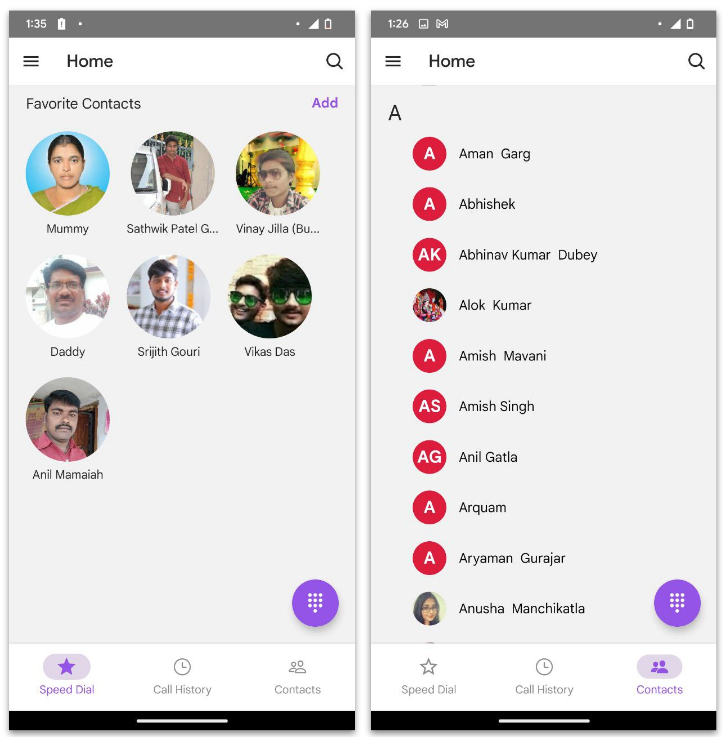
\includegraphics[width=1\linewidth]{Media//demo.png}
    \caption{Demo}
    \label{fig:App demo image}
\end{figure}


\begin{figure}
    \centering
    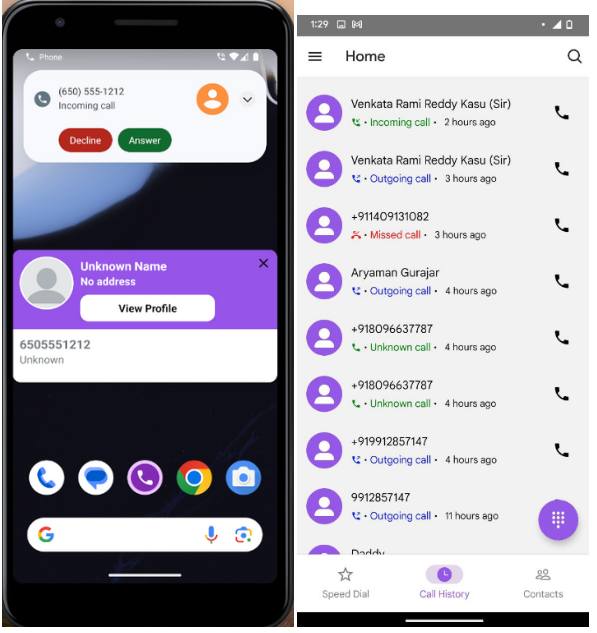
\includegraphics[width=1\linewidth]{Media/demo2.png}
    \caption{Demo 2}
    \label{fig:App Start}
\end{figure}